\documentclass[11pt,oneside]{scrbook}
\usepackage[a4paper,margin=2.4cm,marginparwidth=1.8cm,marginparsep=0.4cm]{geometry}
\usepackage{../common/rlstudy}

\title{{\color{rlblue}\textbf{Week 9} \\ \Huge Proximal Policy Optimization (Deep Dive)}}
\author{STUDY-RL --- a self-paced Deep RL curriculum}
\date{\today}

\begin{document}
\maketitle
\tableofcontents
\newpage

\chapter*{Learning objectives}
\addcontentsline{toc}{chapter}{Learning objectives}


% Teaching companion: a small example before the full lecture.
\noindent\textbf{Study companion.} Read \texttt{teaching\_guide.md} in this
folder for step-by-step examples, an analogy with its limits, and self-checks.
Then use \texttt{workbook.ipynb} to implement and vary the calculations.
\par\medskip

\begin{keyidea}
By the end of this week you will be able to:
\begin{enumerate}[leftmargin=*]
  \item Motivate PPO's clipped surrogate using TRPO's trust-region idea; explain why clipping is a heuristic objective rather than a hard trust-region constraint.
  \item State and implement the PPO-KL variant (adaptive penalty) and contrast its behaviour with PPO-clip.
  \item Recite, implement, and \emph{check off} the 37 implementation details that separate a paper PPO from a working PPO.
  \item Train PPO on BipedalWalker-v3 with vector envs and reproduce the canonical learning curve.
  \item Understand why PPO is the universal workhorse of RLHF and what about its design makes it the right algorithm for LLM fine-tuning (preview of week 18).
\end{enumerate}
\end{keyidea}

\chapter{Motivation and intuition}

TRPO works but is expensive: every update requires a conjugate-gradient solve of $Fx=g$ ($\sim$10 Fisher--vector products), a back-tracking line search, and a separate value-function fit.\marginnote{The Engstrom 2020 paper (week 8 extended reading) showed that the algorithm-vs-code-tricks split is roughly 20--80 in favour of code tricks; this informs the entire structure of this week.} For deep RL at scale, this is a non-starter. PPO is the engineer's compromise: keep the trust-region \emph{idea} (don't move the policy too far per update) but replace the second-order solve with a first-order surrogate that mini-batch SGD can handle, and run multiple epochs of mini-batch updates per rollout.

\begin{intuition}
Picture the importance ratio $\rho_t(\theta) = \Policy_\theta(a_t\given s_t)/\Policy_{\theta_\text{old}}(a_t\given s_t)$. An exact action importance ratio still changes measure correctly at a fixed state, but large ratios increase variance and the old-policy state distribution becomes stale. PPO compares the unclipped and clipped objectives and removes an incentive for further improvement beyond a threshold. It does not constrain every actual ratio to $[1-\varepsilon,1+\varepsilon]$ or guarantee a KL bound.
\end{intuition}

\section*{PPO as the universal workhorse}
PPO is used in continuous-control benchmarks, multi-agent variants such as
MAPPO, and preference training such as InstructGPT. Its first-order update
is convenient, but its performance depends on the implementation, task, and
hyperparameters. Neither clipping nor a commonly used recipe guarantees
robustness or a particular scaling law.

\begin{pitfall}
``It worked in their paper, why doesn't it work for me?'' is almost always one of the 37 details. The two most common: forgetting advantage normalisation (the gradient ends up dominated by a few high-magnitude samples), and forgetting that value clipping needs the \emph{old} value estimate, not the current one.
\end{pitfall}

\chapter{Mathematical formulation}

\section{Importance sampling and the surrogate}

We collect rollouts under $\Policy_{\theta_\text{old}}$, then optimise the importance-sampled objective
\[
  L^{\mathrm{IS}}(\theta) = \E_{(s,a)\sim\Policy_{\theta_\text{old}}}\!\left[\frac{\Policy_\theta(a\given s)}{\Policy_{\theta_\text{old}}(a\given s)} \hat\Adv(s,a)\right] = \E[\rho(\theta)\hat\Adv].
\]
\textbf{Why this is the right surrogate.} Differentiating in $\theta$ at $\theta=\theta_\text{old}$:
\[
  \nabla_\theta L^{\mathrm{IS}}\big|_{\theta_\text{old}}
  = \E\!\left[\frac{\nabla_\theta \Policy_\theta(a\given s)}{\Policy_{\theta_\text{old}}(a\given s)}\big|_{\theta_\text{old}} \hat\Adv\right]
  = \E\!\left[\nabla_\theta \log\Policy_\theta(a\given s)\big|_{\theta_\text{old}} \hat\Adv\right],
\]
which is exactly the policy gradient with advantage $\hat\Adv$. With an appropriate advantage estimator, the surrogate matches the policy-gradient direction at $\theta_\text{old}$. Away from that point it still uses old-policy states and advantages; it is not the exact new-policy return. Clipping discourages large updates without proving a bound on this mismatch.

\section{PPO-clip}

\begin{definition}[PPO clipped surrogate]
\label{def:ppoclip}
With $\rho_t(\theta) \defeq \Policy_\theta(a_t\given s_t)/\Policy_{\theta_\text{old}}(a_t\given s_t)$,
\[
  L^{\mathrm{CLIP}}(\theta) = \E_t\!\left[\min\Big(\rho_t(\theta) \hat\Adv_t,\; \mathrm{clip}(\rho_t(\theta), 1-\varepsilon, 1+\varepsilon) \hat\Adv_t \Big)\right].
\]
\end{definition}

\paragraph{Per-sample analysis.} Fix one $(s_t, a_t)$ with advantage $\hat\Adv_t$. Two cases:
\begin{itemize}[leftmargin=*]
  \item $\hat\Adv_t > 0$ (this action looked good): the surrogate is $\rho_t \hat\Adv_t$ until $\rho_t = 1+\varepsilon$, where it saturates. Above $1+\varepsilon$ the gradient is zero --- ``stop pushing this action's probability higher; we've already increased it enough''.
  \item $\hat\Adv_t < 0$ (this action looked bad): the surrogate is $\rho_t \hat\Adv_t$ until $\rho_t = 1-\varepsilon$, where it saturates. Below $1-\varepsilon$ the gradient is zero --- ``stop pushing this action's probability lower; it's already small enough''.
\end{itemize}
The clip is asymmetric in $\hat\Adv$. The $\min$ makes it a \emph{pessimistic} bound on the surrogate: we never let optimism beyond the clip range drive the update.

\begin{figure}[h]
\centering
\begin{tikzpicture}[scale=0.9]
  \draw[->,thick] (0,0) -- (5,0) node[right]{$\rho_t$};
  \draw[->,thick] (1.5,-2.5) -- (1.5,2.5) node[above]{$L^{\mathrm{CLIP}}_t$ (per-sample)};
  \node at (1.5,-0.25) {$1$};
  \draw[dotted] (1.0,-2.5) -- (1.0,2.5) node[above right, font=\tiny]{$1-\varepsilon$};
  \draw[dotted] (2.0,-2.5) -- (2.0,2.5) node[above right, font=\tiny]{$1+\varepsilon$};
  % Advantage > 0
  \draw[rlblue,thick] (0.3,0.6) -- (2.0,2.0) -- (4.5,2.0);
  \node[rlblue] at (4.3,2.3) {\small $\hat A > 0$};
  % Advantage < 0
  \draw[rlteal,thick] (0.3,-0.5) -- (1.0,-0.5) -- (4.5,-2.25);
  \node[rlteal] at (4.3,-2.3) {\small $\hat A < 0$};
\end{tikzpicture}
\caption{PPO-clip per-sample surrogate as a function of the importance ratio $\rho_t$. The blue (positive advantage) branch flattens above $1+\varepsilon$; the teal (negative advantage) branch flattens below $1-\varepsilon$.}
\end{figure}

\section{PPO-KL (adaptive penalty)}

The original PPO paper also presents
\[
  L^{\mathrm{KL}}(\theta) = \E_t\!\left[\rho_t(\theta) \hat\Adv_t\right] - \beta\, \E_t\!\left[\KL\big(\Policy_{\theta_\text{old}}(\cdot\given s_t)\,\|\,\Policy_\theta(\cdot\given s_t)\big)\right],
\]
with $\beta$ adapted online: if measured KL exceeds the target by $1.5\times$, double $\beta$; if it falls under the target by $0.67\times$, halve it. This is the closest first-order approximation to TRPO's hard KL constraint.

\textbf{Empirical verdict.} Clip wins in practice. KL-penalty is slightly more theoretically clean (Pinsker-based safety angle) but tunes worse out of the box. The exception: RLHF, where the KL term is kept anyway (as a regulariser against reward hacking) and clip is layered \emph{on top} of it.

\section{The full PPO loss}

\[
  L^{\mathrm{PPO}}(\theta, \phi) =
  \underbrace{L^{\mathrm{CLIP}}(\theta)}_\text{policy}
  - c_v\, \underbrace{\E_t\!\left[(\Vfn_\phi(s_t) - \hat R_t)^2\right]}_\text{value}
  + c_H\, \underbrace{\E_t\!\left[\mathcal{H}(\Policy_\theta(\cdot\given s_t))\right]}_\text{entropy bonus}.
\]
With value clipping enabled (detail \#13), the value loss becomes
\[
  L^{\mathrm{V}}(\phi) = \E_t\!\left[\max\Big( (\Vfn_\phi(s_t) - \hat R_t)^2,\; (\mathrm{clip}(\Vfn_\phi(s_t), \Vfn_\text{old} - \varepsilon, \Vfn_\text{old}+\varepsilon) - \hat R_t)^2 \Big)\right].
\]

\chapter{Algorithms}

\begin{tcolorbox}[colback=rlbg, colframe=rlblue, title=\textbf{PPO (Schulman 2017) --- the canonical loop}]
\textbf{Hyper-params:} $N$ vec envs, rollout $T_R = 2048$, mini-batches $M=64$, epochs $K=10$, $\Disc=0.99$, $\lambda=0.95$, $\varepsilon=0.2$, $c_v=0.5$, $c_H = 0.01$, Adam lr $= 3\times 10^{-4}$ (annealed linearly), grad-clip $0.5$.\\
\textbf{Repeat:}
\begin{enumerate}[leftmargin=*]
  \item Collect $N \times T_R$ transitions under $\Policy_{\theta_\text{old}}$, store $(s, a, r, d, \log\Policy_t^\text{old}, \Vfn_t^\text{old})$.
  \item Bootstrap value for the final state of each env; compute GAE $\hat\Adv_t$ and returns $\hat R_t = \hat\Adv_t + \Vfn_t^\text{old}$.
  \item Standardise $\hat\Adv$.
  \item \textbf{For $k=1,\ldots,K$ epochs:}
    \begin{enumerate}
      \item Shuffle indices; iterate over mini-batches of size $M$.
      \item Compute $\rho_t$, $L^{\mathrm{CLIP}}$, value loss (clipped), entropy bonus; sum into $L^{\mathrm{PPO}}$.
      \item Optionally early-stop if approximate KL $\ge 1.5 \cdot \mathrm{KL}_\text{target}$.
      \item Optimise one Adam step with grad-clip.
    \end{enumerate}
  \item $\theta_\text{old} \leftarrow \theta$, $\Vfn_\text{old} \leftarrow \Vfn_\phi$.
\end{enumerate}
\textbf{Complexity per update:} $\mathcal{O}(N T_R K)$ in transitions; backbone of all modern on-policy RL.
\end{tcolorbox}

\section{The 37 implementation details}

The canonical list (Huang et al., \emph{The 37 Implementation Details of Proximal Policy Optimization}, ICLR Blog 2022 \& \texttt{iclr-blog-track.github.io/2022/03/25/ppo-implementation-details/}) groups details into core, Atari-specific, continuous-control-specific, LSTM, and multi-discrete variants. We list and motivate them.

\begin{table}[h!]
\centering\tiny
\begin{tabular}{lp{8.5cm}l}\toprule
\# & Detail & Category \\ \midrule
1 & Vectorised env (Sync or Async) for parallel rollouts. & core \\
2 & Orthogonal weight init: actor final layer std $0.01$, value head std $1.0$, hidden std $\sqrt{2}$. & core \\
3 & Adam, $\varepsilon=10^{-5}$ (not the default $10^{-8}$). & core \\
4 & Linear learning-rate schedule (decay to zero). & core \\
5 & GAE with $\Disc=0.99, \lambda=0.95$. & core \\
6 & Per-mini-batch advantage normalisation. & core \\
7 & PPO-clip $\varepsilon=0.2$; alternative: clip on the log-ratio. & core \\
8 & Value-function clipping (clip range $\varepsilon$). & core \\
9 & Joint policy+value MSE+entropy loss, weights $1, 0.5, 0.01$. & core \\
10 & Global gradient norm clipping at $0.5$. & core \\
11 & Approximate-KL early stopping at $1.5\cdot\mathrm{KL}_\text{target}$. & core \\
12 & Independent observation/return normalisation (running mean/std). & core \\
13 & Returns clipping (clip to $\pm 10$) for stability with value clipping. & core \\
14 & Reward clipping to $\pm 10$. & core \\
15 & State-independent log-std (continuous). & continuous \\
16 & $\tanh$ activation in the policy (vs.\ ReLU in value). & continuous \\
17 & Initial log-std $0$ (not $-0.5$). & continuous \\
18 & Action clipping to $[-1, 1]$ after sampling. & continuous \\
19 & Frame skip $4$ (Atari) / no skip (continuous). & Atari \\
20 & Frame stack $4$ (Atari). & Atari \\
21 & Greyscale + 84$\times$84 resize (Atari). & Atari \\
22 & ``Fire-on-reset'' action (Atari). & Atari \\
23 & Episodic life wrappers (Atari). & Atari \\
24 & Reward sign clipping (Atari only). & Atari \\
25 & NoOp reset 0--30 steps (Atari). & Atari \\
26 & MaxAndSkipEnv for frame skip (Atari). & Atari \\
27 & Conv-trunk init: orthogonal $\sqrt{2}$. & Atari \\
28 & Final policy head init: orthogonal $0.01$. & core \\
29 & Final value head init: orthogonal $1.0$. & core \\
30 & Mini-batch size $\le$ rollout / 4 (typically). & core \\
31 & $K=10$ epochs (continuous), $K=4$ (Atari). & core \\
32 & Seed all RNGs identically (Python, NumPy, Torch, env). & core \\
33 & Deterministic CUDNN \emph{off} for speed. & core \\
34 & LSTM: \texttt{burn-in} hidden state from rollout for first $T_b$ steps. & LSTM \\
35 & LSTM: zero-out hidden state at episode boundaries. & LSTM \\
36 & Reward-to-go normalisation (alt to advantage normalisation). & alt \\
37 & Mixed-precision off by default (FP32 matters for small policies). & core \\
\bottomrule
\end{tabular}
\caption{The 37 implementation details, distilled from Huang et al.\ 2022. The project's \texttt{train.py} checks off (1)--(18) and (28)--(33).}
\end{table}

\chapter{Implementation walkthrough}

The trainer retains the sampled Gaussian latent action for its likelihood;
only the action sent to the environment is clipped to the action-space bounds.
Scoring a clipped action as the original draw would invalidate likelihood ratios.
A true terminal removes the value bootstrap, while a time-limit truncation
bootstraps from the final observation and stops the GAE trace before the
reset episode. The common rollout helpers request same-step autoreset and
recover the final observation supplied in its info dictionary.


\section{Vector env + GAE collection (details 1, 5, 6, 12)}

\begin{minted}{python}
envs = gym.vector.SyncVectorEnv(
    [lambda i=i: gym.wrappers.NormalizeObservation(
                  gym.wrappers.NormalizeReward(gym.make(env_id, autoreset=True)))
     for i in range(num_envs)])
\end{minted}

\section{PPO loss (details 7, 8, 9, 11)}

\begin{minted}{python}
def ppo_loss(logp, logp_old, value, value_old, advantages, returns,
             clip_eps=0.2, value_coef=0.5, entropy_coef=0.01,
             entropy=None):
    ratio = torch.exp(logp - logp_old)
    surr1 = ratio * advantages
    surr2 = torch.clamp(ratio, 1 - clip_eps, 1 + clip_eps) * advantages
    pi_loss = -torch.min(surr1, surr2).mean()

    v_clipped = value_old + torch.clamp(value - value_old, -clip_eps, clip_eps)
    v_loss1 = (value - returns) ** 2
    v_loss2 = (v_clipped - returns) ** 2
    v_loss = 0.5 * torch.max(v_loss1, v_loss2).mean()

    H = entropy.mean() if entropy is not None else torch.tensor(0.0)
    loss = pi_loss + value_coef * v_loss - entropy_coef * H

    approx_kl = (logp_old - logp).mean()
    return loss, pi_loss, v_loss, H, approx_kl
\end{minted}

\section{Linear LR schedule + Adam $\varepsilon=10^{-5}$ (details 3, 4)}

\begin{minted}{python}
opt = torch.optim.Adam(net.parameters(), lr=3e-4, eps=1e-5)
for it in range(n_iters):
    frac = 1.0 - it / n_iters
    for g in opt.param_groups:
        g["lr"] = 3e-4 * frac
\end{minted}

\chapter{Empirical results}

\begin{figure}[h]
\centering
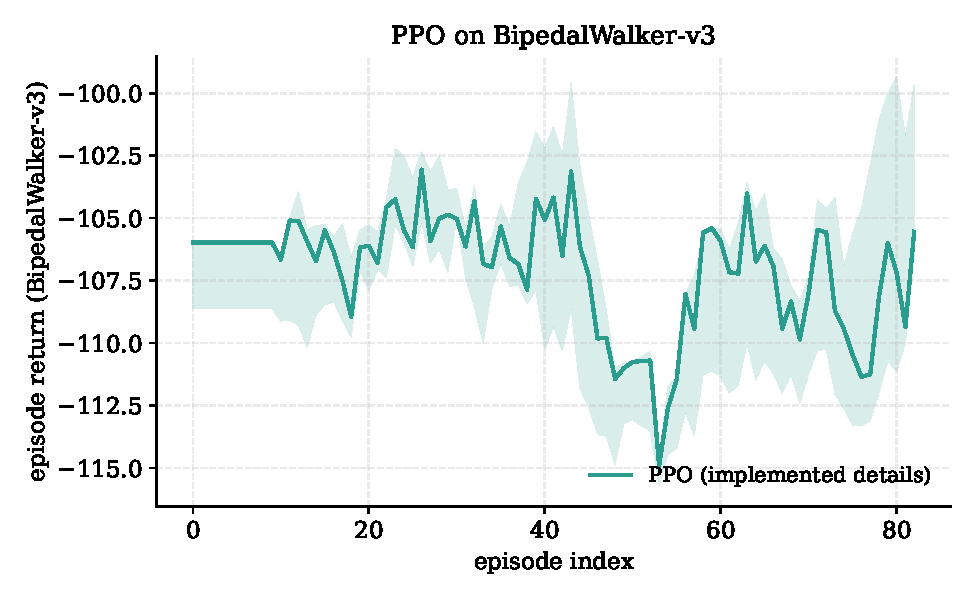
\includegraphics[width=0.85\linewidth]{figs/ppo_walker.pdf}
\caption{PPO on BipedalWalker-v3. Mean and IQR over 3 seeds, $N=8$ vec envs, $T_R=512$, $K=4$ epochs, $\varepsilon=0.2$.}
\label{fig:ppo-walker}
\end{figure}

\begin{figure}[h]
\centering
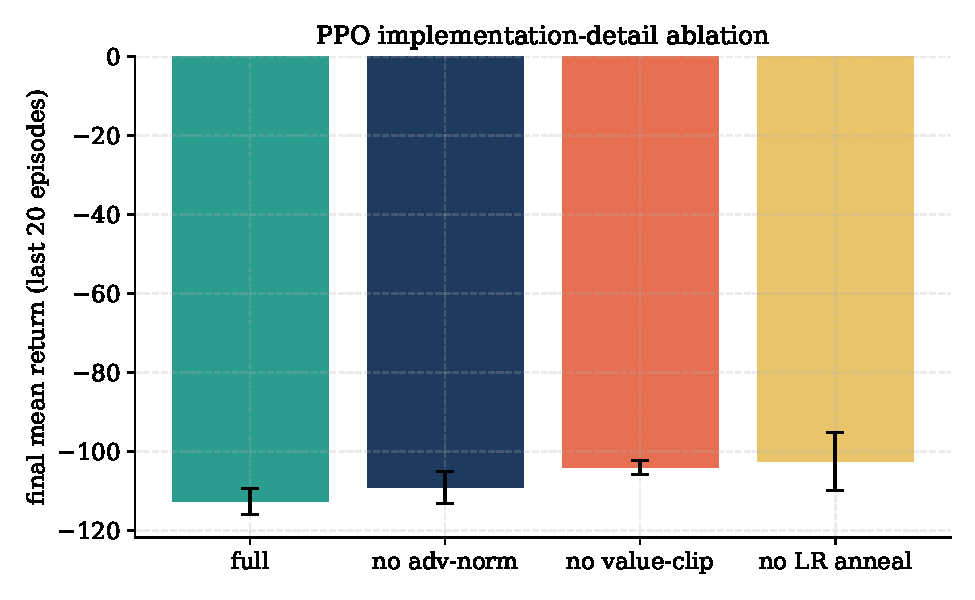
\includegraphics[width=0.85\linewidth]{figs/details_ablation.pdf}
\caption{The cost of skipping details: PPO with vs.\ without advantage normalisation (\#6), value clipping (\#8), and learning-rate annealing (\#4). Effects and ordering need not transfer to another task or budget.}
\label{fig:details-ablation}
\end{figure}

\chapter{Safety angle}

\begin{safetyangle}
\textbf{PPO is the algorithm of RLHF.} Stiennon et al.\ 2020 and Ouyang et al.\ 2022 both use PPO as the RL backbone. The KL penalty between $\Policy_\theta$ and the SFT reference $\Policy_\text{ref}$ is added to the reward signal:
\[
  r_\text{shaped}(s, a) = r_\text{RM}(s, a) - \beta\, \log \frac{\Policy_\theta(a\given s)}{\Policy_\text{ref}(a\given s)}.
\]

\paragraph{Two different anchors.} PPO clipping discourages excessive improvement on sampled actions relative to the rollout policy. It does not bound per-step or total KL: shared parameters and other samples can move an already-clipped ratio further. The KL-to-SFT-reference reward penalty serves a separate purpose and a different reference distribution. Monitor both divergences; neither a finite penalty nor clipping alone is a hard safety constraint.

\paragraph{Failure modes (concrete).}
\begin{enumerate}[leftmargin=*]
  \item \textbf{Reward over-optimisation.} Gao--Schulman--Hilton 2022 (arXiv:2210.10760) show RLHF's proxy reward gap grows quadratically in $\sqrt{\KL}$ from the SFT. Mitigation: KL-penalty (above), early stopping by KL.
  \item \textbf{Mode collapse / repetition.} Removing the entropy bonus collapses LLM outputs to a few canned responses. Mitigation: keep $c_H \ge 0.001$ even at the cost of slightly lower reward-model score.
  \item \textbf{Distribution shift in the value head.} The value net is trained on $\Policy_\text{old}$ rollouts; if $\Policy$ moves too fast, $\Vfn_\phi$ is stale and advantages are biased. Mitigation: lower learning rate, more epochs to fit $\Vfn$ relative to $\Policy$.
  \item \textbf{Spec-gaming by clip exploitation.} If a state has hugely positive advantage and $\rho_t$ jumps above $1+\varepsilon$ before the gradient saturates, you can still get a destructive update. Mitigation: detail \#11 (KL early stopping).
\end{enumerate}

A preview of week 18: every one of these failure modes will reappear when we train PPO on a Pythia-160M with LoRA, and the mitigations are identical.
\end{safetyangle}

\chapter{Matching application}

\begin{matching}
\textbf{PPO as the slate-ranking optimiser for synthetic ATS / synthetic insurance.}

The leap from REINFORCE-for-ranking (week 7) to PPO-for-ranking is modest: replace the single-update gradient step with the PPO-clip surrogate over a mini-batch of logged slates, run for $K=4$ epochs, and apply value-function clipping. The benefits:
\begin{itemize}
  \item \textbf{Stability under reward-model drift.} A click-through-rate proxy reward $r_\text{RM}$ that gets re-trained nightly cannot induce a runaway optimiser; PPO-clip discourages large updates, while measured KL and independent evaluation remain necessary.
  \item \textbf{Mini-batch parallelism.} The same logged batch supports multiple SGD steps; you extract roughly $4\times$ the gradient signal per data unit relative to REINFORCE.
  \item \textbf{Direct KL audit.} The approximate-KL metric is logged at every update; an alarm at $\KL > 0.05$ catches a misbehaving update before it ships.
\end{itemize}

\paragraph{Concrete recipe for synthetic insurance weekly retrains.}
\begin{enumerate}
  \item Collect last 7 days of logged slates with behaviour-policy probabilities.
  \item Check logger coverage and propensity accuracy; SNIPS estimates policy value, not a canonical per-transition advantage. Reusing historical logs requires a separately justified off-policy learning objective (week 11).
  \item PPO-clip update: 4 epochs, $\varepsilon=0.1$ (tighter than the standard 0.2 because logged data has more importance-ratio variance), early-stop on KL$>10^{-2}$.
  \item Online A/B with the new $\theta$ for 48 hours; gate the rollout on a CTR-improvement test and a slot-share-stability check.
\end{enumerate}
This is an application sketch, not an established universal recipe: PPO normally refreshes data from its current rollout policy, and stale logged slates require additional off-policy reasoning.
\end{matching}

\chapter{Exercises}

\begin{enumerate}[label={},leftmargin=0pt,labelsep=0pt]
  \item \textbf{E1} ($\star$) Implement \texttt{ppo\_clip\_loss(ratio, adv, eps)} and unit-test edge cases.
  \item \textbf{E2} ($\star$) Show that $L^{\mathrm{CLIP}}$ is differentiable everywhere except $\rho \in \{1-\varepsilon, 1+\varepsilon\}$ and explain why this is fine in practice.
  \item \textbf{E3} ($\star\star$) Implement value-function clipping; show that disabling it degrades final return on a 50-update toy.
  \item \textbf{E4} ($\star\star$) Train PPO on BipedalWalker-v3; reach mean return $\ge 100$ within 800 updates.
  \item \textbf{E5} ($\star\star$) Ablate three details from the 37; produce Figure~\ref{fig:details-ablation}.
  \item \textbf{E6} ($\star\star$) Compute the empirical KL between $\Policy_\theta$ and $\Policy_{\theta_\text{old}}$ each update; verify the KL early-stop fires sensibly.
  \item \textbf{E7} ($\star\star\star$) Implement PPO-KL (adaptive penalty) and compare to PPO-clip head-to-head.
  \item \textbf{E8} ($\star\star\star$, meaningful objective) Add a $-\beta \KL(\Policy\|\Policy_\text{ref})$ term to the reward (RLHF-style); show that with $\beta > 0$ the policy stays within a small KL ball of $\Policy_\text{ref}$ even when the reward model is biased.
\end{enumerate}

\chapter{Further reading}

See \texttt{extended\_reading.pdf}. Five papers: Schulman et al.\ 2017 (PPO), Huang et al.\ 2022 (37 details blog \& ICLR poster), Engstrom et al.\ 2020 (Implementation Matters), Andrychowicz et al.\ 2021 (\emph{What Matters in On-Policy RL?}), and Ouyang et al.\ 2022 (InstructGPT --- PPO for RLHF). Sourced from \texttt{research/deeprl\_core\_sota.md} \S 2.6 and \texttt{research/llm\_rl\_sota.md}.

\end{document}
